\documentclass[conference]{IEEEtran}
\IEEEoverridecommandlockouts
% The preceding line is only needed to identify funding in the first footnote. If that is unneeded, please comment it out.
\usepackage{cite}
\usepackage{amsmath,amssymb,amsfonts}
\usepackage{algorithmic}
\usepackage{graphicx}
\usepackage{textcomp}
\usepackage{xcolor}
\usepackage{float}
\usepackage{kotex}


\def\BibTeX{{\rm B\kern-.05em{\sc i\kern-.025em b}\kern-.08em
    T\kern-.1667em\lower.7ex\hbox{E}\kern-.125emX}}
\begin{document}

\title{Farm Product Price Inform Service – NUGU FRESH \\
\thanks{Identify applicable funding agency here. If none, delete this.}
}
\author{\IEEEauthorblockN{Kim Kwang Yeon}
\IEEEauthorblockA{\textit{Department of Information Systems} \\
\textit{College of Engineering}\\
Hanyang University\\
Seoul, Rep. of Korea \\
Email: kwang9705@gmail.com}
\\
\IEEEauthorblockN{Kim Jin Hyeok}
\IEEEauthorblockA{\textit{Department of Information Systems } \\
\textit{College of Engineering}\\
Hanyang University\\
Seoul, Rep. of Korea\\
Email: wlsgur948861@gmail.com
}
\\
\and
\IEEEauthorblockN{Kim Bong Kyun}
\IEEEauthorblockA{\textit{Department of Information Systems } \\
\textit{College of Engineering,}\\
Hanyang University\\
Seoul, Rep. of Korea\\
Email: qhdrnak@gmail.com }
\\
\IEEEauthorblockN{Choi Hyun Ji}
\IEEEauthorblockA{\textit{Department of Information Systems } \\
\textit{College of Engineering,}\\
Hanyang University\\
Seoul, Rep. of Korea\\
Email: tomz.seras@gmail.com}
}


\maketitle

\begin{abstract}
For decades, government has been seeking solutions by setting price stability of agricultural products as its top priority. However, according to Ministry of Food and Drug Safety, crops with high consumer demand, such as potatoes and cabbage, are experiencing price fluctuations every two to three years due to various causes such as rising consumer prices and imports. In recent years, natural disasters such as floods and droughts have frequently occurred due to rapid changes in the climate environment, and as a result, the volatility of agricultural product prices is increasing more. Also, Fresh product delivery services have continued to increase due to the explosive increase in non-face-to-face delivery services since the COVID-19 incident and the prices fluctuate frequently and vary from company to company. At these reasons, NUGU Fresh was developed in consideration of the situation of agricultural products with such high price volatility. For those who often use early morning delivery, such as students living alone or those who don’t want to go and buy themselves, the prices of various companies’ early morning delivery crops are compared to the prices of marts and markets, and housewives and agricultural wholesalers can check the current market price and future price trends of agricultural products through NUGU speakers. In addition, sellers in traditional markets who are vulnerable to information can set standards for what prices to sell agricultural products.
\end{abstract}

\section{Introduction}
\subsection{Motivation}
In recent years, prices of major agricultural products have soared along with rising consumer prices and natural disasters, causing inconvenience to consumers. For one example, typhoon damage occurs frequently from July to October when there is a holiday called Chuseok in Korea. In addition, when Chuseok approaches, most families buy holiday food ingredients, so consumer prices rise a lot. If a typhoon comes during this period, consumer prices can jump unimaginably. If this situation occurs, consumers may feel a great burden on prices. In anticipation of such impacts as natural disasters and increased demand, the government strives to stabilize prices by supplying more raw materials to the market to control prices. These supply and demand stabilization policies were promoted as a way to reduce the risk of price fluctuations, but detailed analysis is insufficient. Accurate analysis of how specific the price will change is still poor and decisions are made based on past experiences. If a high-accuracy agricultural product price prediction model could be created, it would be helpful to prepare in advance by predicting the section where these prices change severely.

\begin{figure}[!htbp]
\centering
    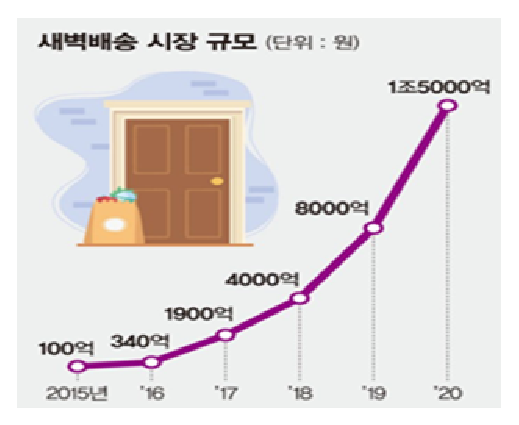
\includegraphics[width =6cm]{pictures/picture1.eps}
    \hfil
\caption{Early morning delivery market size}
\label{Early morning delivery market siz}
\end{figure}

In addition, this prediction model is expected to help a lot at the personal level. Currently, many stories of housewives or wholesalers who are worried about agricultural prices are being introduced in the news. Housewives or wholesalers are often less familiar with electronic devices such as smartphones than younger people. In particular, elderly sellers who sell goods in traditional markets are bound to be more vulnerable to such price information. Currently, this agricultural price information can be found on a somewhat unfamiliar website called KAMIS. It only presents current and past prices here, but does not provide predictions of what future price information will be. Looking at this point, we wanted to create a service through artificial intelligence speakers that answers price information without complicated settings or access processes, and creating a homepage that can visualize and print such data to help these people. Housewives will be able to get a rough idea of when to buy agricultural products, and wholesalers will be able to set standards for what price to sell products in the coming future.

\begin{figure}[!htbp]
\centering
    
\includegraphics[width =6cm]{pictures/picture2.eps}
    \hfil
\caption{Increase in users of early morning delivery}
\label{Increase in users of early morning delivery}
\end{figure}

Moreover, Fresh product delivery services have continued to increase due to the explosive increase in non-face-to-face delivery services since the COVID-19 incident. These services are very popular not only among young people, but also among middle-aged people between 50 and 60. According to a news article by ITWORLD, only 52\% of middle-aged people had experience using fresh products delivery in 2022 and nearly half of them used service frequently. Although the number of people using fresh product delivery services is increasing, there was no platform to compare the price of fresh product delivery sold by each company. In view of this inconvenience, we tried to provide the price information by NUGU speaker which is easy to access. As for the brands to compare prices, the representative brands of the three companies (Coupang Gomgom, Market Kurly KF365, SSG FRESH) and the average price of the mart and market provided by KAMIS were selected. Fresh products included in the top 30 heavily consumed foods selected by MFDS in Korea were chosen as the targets for price comparison. Through these services, At the same time, by predicting the prices of these fresh products, we intended to make it easier for consumers to choose by informing the trend of the prices of fresh products so that the timing of purchase could be determined easily.




\subsection{Research on any related software}
\subsubsection{NUGU coin}

NUGU Coin service provides real-time coin market price information of the virtual asset exchange Bithumb. Coin information such as Bitcoin, Ethereum, and Ripple can be known, but market price errors may occur due to network and server failures.
\subsubsection{Ustockplus Chart Prediction Service}
The Ustockplus Chart Prediction Service analyzes past charts to predict the current most likely pattern and draws the predicted stock price on the stock chart. Ustockplus Chart Prediction Service analyzes the previous data statistically through its own prediction algorithm.
\subsubsection{Farm Morning}
Farm Morning notifies the national market price of agricultural products in real time. Farmers can immediately calculate how much they can earn from agricultural products harvested on the same day, so they can check the market price and sell agricultural products under the best conditions. It also provides weather information and cultivation information necessary for farming.\\

\begin{table}[!htbp]
\caption{ROLE ASSIGNMENTS}
\begin{tabular}{|c|c|p{2.5cm}|}
\hline
Roles& Name & Task descrption and etc\\
\hline 
user&Choi Hyun Ji & No matter how good the system is, it is meaningless if it is not easy to use from the user's point of view. He considers whether these services are easily accessible. If not, it suggests a way to develop service quality easily.\\
\hline
Customer& Kim Kwang yeon &Analyze the service from the buyer's point of view. Design services in consideration of appropriate costs and resources, and organize services to reach consumers attractively. \\
\hline
Software Developer & Kim Bong Kyun & Software developers design a full-scale software configuration. Write overall code without errors, and make the application do some tasks.\\
\hline
Development Manager& Kim Jin Hyeok & The development manager determines the overall software development process and appropriately distributes the schedule for each process. It also makes development easier by presenting tools that can be useful in the development process\\
\hline
\end{tabular}
\end{table}

\section{REQUIREMENTS}
\subsection{NUGU Speaker }\label{AA}
\subsubsection{Price notification service}
\paragraph{return historic market price}
You can know the past price of agricultural products through AI speakers. First, the user commands the speaker to “Start NUGU Fresh” or “Please turn on NUGU FRESH”. The speaker then gets the command, “It’s NUGU Fresh. What can I help you?” To know the price, two characteristics are required: crop name and date, and if any of them are not met, the AI speaker does not return the price. NUGU FRESH handles five crops which were ranked as the most consumed by  MFDS in Korea: potato, cabbage, radish, rice, and onion. When user asks for other crops, then NUGU FRESH will say “It’s a request that cannot be processed. Please tell me again.” Moreover, for example, if a user says, “Tell me the price of cabbage,” the AI speaker asks back, “Please tell me the date”, and if the user tells “a week ago,” then the speaker tells you the difference between the cabbage price and the cabbage price at the time of ignition a week ago. When returning the historic market price, NUGU FRESH will say “The price of radish on last week was OOO won. Current price is OOO won and this is an increase of OO won compared to the historic price”.
\paragraph{Return current market price}
Similar to returning historic market price, user has to satisfy two elements: crop name, and date. If user says, “Tell me the today’s price of rice”, NUGU FRESH will answer “Today’s price of rice is OOO won”

\paragraph{Forecasting future market prices}
After satisfying the two elements, the command tells you the future predictors. However, future predictions can be made up to a week. When a user says, “Tell me the price of cabbage in a year”, it returns “It’s a request that cannot be processed. Please tell me again”. When returning the future forecast, predicting price fluctuations through differences from the current price, “The price of radish on next week is expected to be OOO won. This is an increase of OO won compared to the current forecast”.  As such, the direction of the market price of the relevant agricultural product is returned together.

\subsubsection{Early Morning Delivery Price Comparing Service}
\begin{paragraph}{Comparing Delivery Prices}
After NUGU FRESH tells the price of requested crop, AI speaker asks “Do you want to know about early morning delivery price of the crop?” If user says ‘yes’, then the early morning delivery price standard tells you the cheapest of the three companies Coupang Gomgom, Market Kurly KF365, and SSG FRESH, which are the most dominant companies in the early morning delivery industry. For example, when a user asks, "Tell me the today’s price of cabbage," the AI speaker will tell the user today’s price of cabbage and compares the price of cabbage delivered at dawn by the three companies, and then speaks, "The cheapest price of cabbage by early morning delivery is OOO won, and it’s by Coupang. If the user says “No”, then AI speaker just ask about messaging service, and when the user says “Again”, then AI speaker repeats the today’s price of cabage and ask about the early morning delivery service again like above.
\end{paragraph}
\newline
\subsection{Additional Functions}
\subsubsection{Message sending service}
After NUGU FRESH tells the early morning delivery price of the requested crop, AI speaker asks ‘Do you want me to text you the information so far?’ If user answers ‘yes’, it says “I send message to OOO(user name). From now on, shut down NUGU FRESH. Thanks,” and turns off NUFU FRESH. When user answers ‘no’ for the messaging suggestion, AI speaker answers like “From now on, shut down NUGU FRESH. Thanks”, and turns off NUGU Fresh.
\subsubsection{Setting speed of speech}
Adding an in-sentence speech option tag allows users to communicate smoothly with NUGU. Since NUGU Farm is designed for housewives or information-vulnerable groups rather than young people in their 20s and 30s, it sets the utterance speed set to 100\% default to 85\% of NUGU's lowest recommended speed. In addition, before informing the price it creates an environment where users can focus more on the price by setting small period of term before price information through the strong attribute.

\section{DEVELOPMENT ENVIRONMENT}
\subsection{Choice of Software Development Platform}
\subsubsection{Programming Language}
\begin{figure}[!htbp]
\centering
    
\includegraphics[width =4.5cm]{pictures/python}
    \hfil
\caption{python}
\label{python}
\end{figure}

{a)	Python\\
-	Python is high-level programming language which is interpreted and object-oriented. Easy to learn and use Python, which is useful for readability, reduces program maintenance costs. Python supports a variety of modules and packages and pursues program modularization. In particular, it is widely used in data-related fields, supporting modules related to data-specific such as Pandas and Numpy.}

\subsubsection{Development Environment}

\begin{figure}[!htbp]
\centering
    
\includegraphics[width =4.5cm]{pictures/django}
    \hfil
\caption{Django}
\end{figure}
a)	Django\\

-	Django is an advanced Python web framework which pursues practical design and efficient development. Many of the features already created, such as Django Admin, Form, and Serializer, deal with much of the inconvenience of web development, so you don't have to recreate the new features from scratch, just use them. You can also save money as a free open source.

\begin{figure}[!htbp]
\centering
    
\includegraphics[width =4.5cm]{pictures/keras}
    \hfil
\caption{Keras}
\end{figure}
b)	Keras
-	Keras is a deep learning API designed to be human-friendly rather than machine-friendly. Keras was born with great effort to reduce cognitive load. Provides a simple, consistent API, and provides clear, actionable error messages. It also includes a wide range of user manuals, making it easier for users to use.
\begin{figure}[!htbp]
\centering
    
\includegraphics[width =4.5cm]{pictures/airflow.eps}
    \hfil
\caption{Airflow}
\end{figure}

c)	Airflow
-	Apache Airflow is an open-source workflow management platform created for data engineering pipelines. This allows you to manage and monitor complex workflows. It uses directed acyclic graphs (DAGs) to manage workflow coordination. Then, it manages scheduling and execution that can be executed by a defined schedule.

\begin{figure}[!htbp]
\centering
    
\includegraphics[width =4.5cm]{pictures/ncp.eps}
    \hfil
\caption{Naver Cloud Platform}
\end{figure}

d)	Naver Cloud Platform
-	Naver Cloud Platform is an enterprise cloud service provided by Naver Cloud. From basic IaaS such as servers and storage to PaaS, and SaaS, a business collaboration platform such as WORKPLACE. Naver affiliates such as Line, Naver Webtoon, and V-Live are using Naver Cloud Platform, and many large companies have also introduced Naver Cloud Platform services.

\begin{figure}[!htbp]
\centering
    
\includegraphics[width =4.5cm]{pictures/AWS.eps}
    \hfil
\caption{AWS}
\end{figure}
e)	Amazon Web Services
-	Amazon Web Services (AWS) platform provides more than 200 fully featured services from data centers located all over the world, and is the world's most comprehensive cloud platform. It provides scalable and cost-effective cloud solutions such as computer power, database storage, content delivery, etc. 

\begin{figure}[!htbp]
\centering
    
\includegraphics[width =4.5cm]{pictures/github.eps}
    \hfil
\caption{GitHub}
\end{figure}

f)	GitHub
-	GitHub is a web-based version-control and collaboration platform for software developers. Git is used to store the source code for a project and track the complete history of all changes to that code. It allows developers to collaborate on a project more effectively by providing tools for managing possibly conflicting changes from multiple developers.

\begin{figure}[!htbp]
\centering
    
\includegraphics[width =4.5cm]{pictures/nuguplaybuilder.eps}
    \hfil
\caption{Nugu Play Builder}
\end{figure}

g)	NUGU Play Builder
-	NUGU play is a unit of service in response to a user's request through the NUGU platform, and you can create Play in the Play Builder. It helps companies or individuals with good content to provide their services to NUGU users through Play. The User Utterance Model, which understands the user's speech, and then identifies the user's Intent and combines actions that perform functions based on it to create a complete play.

\begin{figure}[!htbp]
\centering
    
\includegraphics[width =4.5cm]{pictures/twilio.eps}
    \hfil
\caption{Twillo}
\end{figure}
h)	Twilio
-	Twilio is a US cloud communication platform as a service (CPaaS) that allows software developers to semi-automatically build business communication processes. Twilio helps its clients focus on their current goals, like communication with partners, customers, and employees instead of spending a huge amount of time negotiating with mobile operators to solve communication problems.\\


\subsection{Cost Estimation}

\begin{table}[!htbp]
\begin{tabular}{|c|l|l|}
\hline
\multicolumn{1}{|l|}{Service}                                     & Region & Cost(hourly) \\ \hline
\begin{tabular}[c]{@{}c@{}}Amazon   \\ EC2 p3.2xlarge\end{tabular} &
  \begin{tabular}[c]{@{}l@{}}North   East\\    \\ (Seoul)\end{tabular} &
  3.06 USD \\ \hline
\begin{tabular}[c]{@{}c@{}}Naver   \\ Ncloud Compact\end{tabular} & Korea  & 48   KRW     \\ \hline
\begin{tabular}[c]{@{}c@{}}Amazon   \\ RDS\end{tabular} &
  North   East (Seoul) &
  \begin{tabular}[c]{@{}l@{}}Cost   is required \\ after 750 hours\end{tabular} \\ \hline
\end{tabular}
\end{table}

\subsection{Development Environment Description}
\begin{table}[h]
\begin{tabular}{|c|c|p{2.5cm}|}
\hline
Name   & Version       & Description                  \\ \hline
Windows            & 10 Home & graphical operating system   developed and published by Microsoft.  \\ \hline
Ubuntu & 16.04 (64bit) & Linux-based operating system \\ \hline
Visual Studio code & 1.72    & Source-code editor made by   Microsoft with the Electron Framework, \\ \hline
\end{tabular}
\end{table}


\subsection{Software in use}
There are websites that compare the prices of various products such as Danawa and Enuri. However, these websites did not directly compare the prices of Coupang, Market Kurly, and SSG, the most popular fresh product delivery platforms. It also did not show what trend prices will change in the future. By comparing these fresh product deliveries to the average price sold at the mart, our NUGU farm make consumers to choose the right choice, and by asking the speaker questions without having to bother comparing directly from the mobile phone through the website.\\

\subsection{Task Distribution}

\begin{table}[h]
\begin{tabular}{|l|l|}
\hline
Name           & Task description   \\ \hline
Kim Kwang Yeon & Play Builder,   AI \\ \hline
Kim Jin Hyeok  & Backend, AI        \\ \hline
Kim Bong Kyun  & Backend, AI        \\ \hline
Choi Hyun Ji   & Play Builder,   AI \\ \hline
\end{tabular}
\end{table}
Basically, each group of two is in charge of one part each.  


\section{Specification}
{
\begin{figure}[!htbp]
\centering
    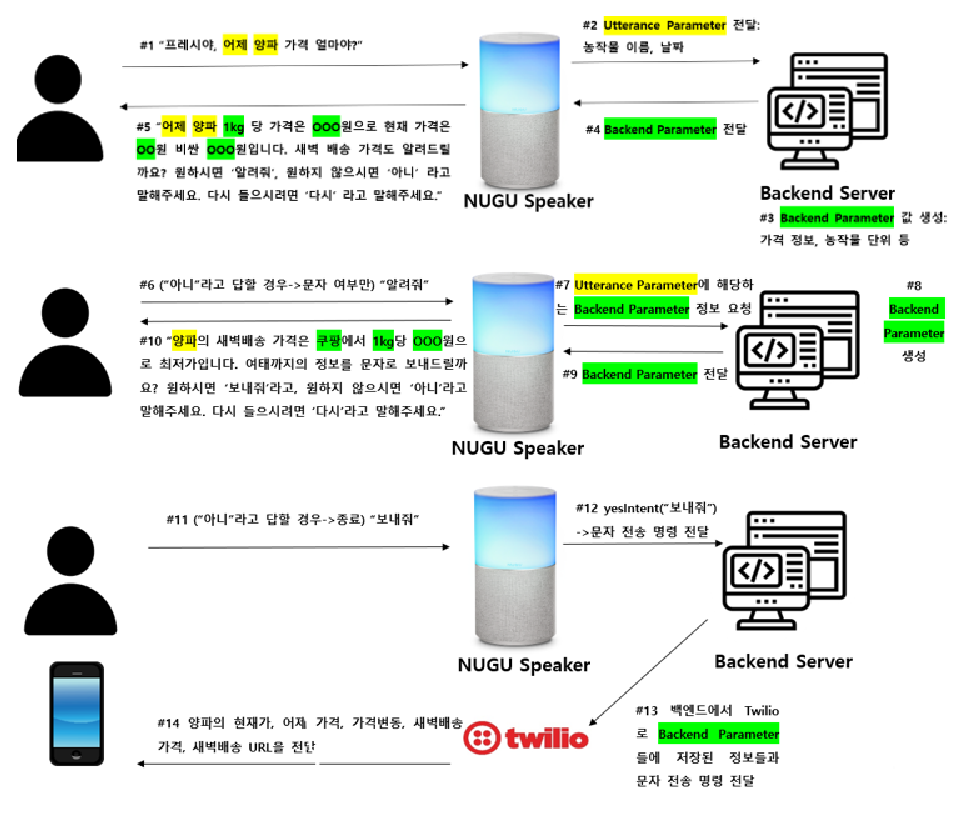
\includegraphics[width =4.5cm]{pictures/picture3.eps}
    \hfil
\caption{Service Scenario}
\label{Service Scenario}
\end{figure}
}

\subsection{NUGU Speaker}

\subsubsection{Price notification service}
\paragraph{ Return historic market price:}
When the user asks to start NUGU farm “프레시 시작”, or “프레시 시작해줘”, the AI speaker will ask “안녕하세요,누구프레시입니다.무엇을도와드릴까요?” The user ask price of crops he wants. At this time, AI Speaker requires two characteristics: crop name, and date. The types of crops include rice, cabbage, onions, radishes, and potatoes, which were selected as most consumed for Koreans by MFDS in Korea. When you ask about other crops, AI speaker says “처리할 수 없는 발화입니다. 다시 말해주세요” Likewise, if the user doesn’t include date, AI Speaker says “날짜를 말해주세요.” These error messages are repeated up to three times, and the AI speaker is terminated “날짜는 필수 요소입니다. 이상으로 누구 프레시를 종료합니다. 감사합니다.” if the conditions are not met after this. Historical data is available up to a week ago. If the user asks “어제 쌀 가격 알려줘,” then AI speaker answers requested crops’ price, and difference between price of yesterday and the point of utterance at that time “쌀의 어제 가격은 OOO원으로 현재는 O 원 비싼 OOO원 입니다.”

\paragraph{Return current market price}
Similar to returning historic market price, user has to satisfy two elements: crop name, and date. After satisfying the three characteristics, the AI speaker tells you the future predictors. If the user asks “오늘 배추 가격 알려줘”, AI speaker answers “오늘 서울 배추의 가격은 OOO원 입니다.” As such, the direction of the market price of the relevant agricultural product is returned together.

\paragraph{Forecasting future market prices}
After satisfying the two characteristics, the AI speaker tells you the future predictors. If the user asks “내일 양파 가격 알려줘”, AI speaker answers “양파의 내일 가격은OOO원으로 예측되고 현재는 OO원 비싼 OOO 원 입니다.” However, NUGU farm can only possible to predict up to a week, so when the user asks price after a week, AI speaker says “처리할 수 없는 요청입니다. 다시 말해주세요.” As such, the direction of the market price of the relevant agricultural product is returned together.
\subsubsection{Early Morning Delivery Price Comparing Service\\}
\paragraph{Comparing Delivery Prices}
After NUGU FRESH tells the price of requested crop, AI speaker asks “새벽 배송 가격도 알려드릴까요? 원하시면 ‘알려줘’, 원하지 않으시면 ‘아니’ 라고 말해주세요. 다시 들으시려면 ‘다시’ 라고 말해주세요.” If user says “알려줘”, then the early morning delivery price standard tells you the cheapest of the three companies Coupang Gomgom, Market Kurly KF365, and SSG FRESH, which are the most dominant companies in the early morning delivery industry. Then AI speaker says “배추의 새벽 배송 가격은 OO(새벽 배송 회사)에서 OOO 원으로 최저가입니다.” Like this, NUGU FRESH compares the prices of early morning delivery services of the three companies "Coupang," "Market Curly" and "SSG.COM" and returns the prices of the cheapest one to users. If the user says “아니”, then AI speaker just ask about messaging service, and when the user says “다시”, then AI speaker repeats the today’s price of cabage and ask about the early morning delivery service again like above. 

\subsubsection{Additional Function}
\paragraph{Setting speed of speech}
When you convert a NUGU speaker's response prompt to voice, you can make it read the way you want it. NUGU speaker is made for the vulnerable, primarily the elderly. The ignition speed was defaulted to the lowest recommended speed of 85\%. You can also adjust the pitch. The pitch is 100\% basic, and the parts that need to be emphasized such as price and product name are set at 105\%. You can adjust the length of silence after reading the sentences, and the main information such as price and product name has increased the existing 300ms to 500ms. By highlighting the key words, the information can be communicated even if the user does not understand the whole context.

\subsection{Message sending service}
\begin{figure}[h]
\centering
    
\includegraphics[width =4.5cm]{pictures/M1.eps}
    \hfil
\end{figure}

\begin{figure}[h]
\centering
    
\includegraphics[width =4.5cm]{pictures/M2.eps}
    \hfil
\end{figure}
\begin{figure}[h]
\centering
    
\includegraphics[width =4.5cm]{pictures/M3.eps}
    \hfil
\caption{Message sending service}
\end{figure}
\newpage

At the end of conversation between NUGU AI speaker and user, AI speaker asks “여태까지의 정보를 문자로 보내드릴까요? 원하시면 ‘보내줘’라고, 원하지 않으시면 ‘아니’라고 말해주세요. 다시 들으시려면 ‘다시’라고 말해주세요.” If user answers “보내줘” and if the user's phone number is already registered, it immediately sends a message containing the price information so far and says “OOO(유저이름) 님에게 문자를 보내드렸어요. 이상으로 누구 프레시를 종료합니다. 감사합니다.” The example message will be like Fig. 10 below. When user answers “아니” for the messaging suggestion, AI speaker answers like “이상으로 누구 프레시를 종료합니다. 감사합니다.” and turns off NUGU Fresh, and when the user says “다시” for the message suggestion, AI speaker will tell the early morning delivery price of the requested crop again and also suggest messaging service like above.



\section{ARCHITECUTRE DESIGN}
\subsection{Overall Architecture}
\begin{figure}[h]
\centering
    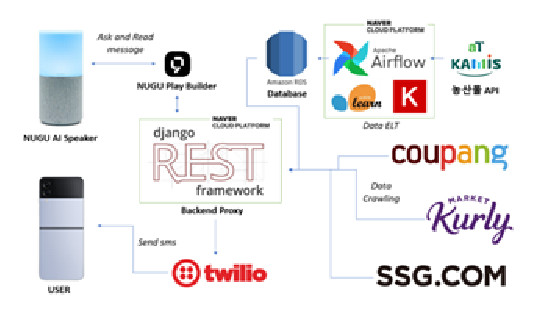
\includegraphics[width =4.5cm]{pictures/structure.eps}
    \hfil
\caption{structure}
\end{figure}
NUGU FRESH is divided in to two main modules: the Backend and the Airflow. 
a) Backend: The backend server has two endpoints (NUGU Play Builder, Twilio). It runs on Naver Cloud, configured using the Django REST framework, and delivers values received from the KAMIS API and values crawled from coupang, kurly, and SSG to NUGU play builder as a response and interacts with users. The Django server finally sends the values so far to the user by text using the Twilio platform.
b) Airflow: Airflow automates the process of extracting data from APIs, preprocessing data using sklearn's minmaxscaler, predicting data using keras' model, and loading the predicted data into a database consisting of AWS RDS. Airflow is running on NAVER CLOUD PLATFORM.

\subsection{Database Design}
\begin{figure}[!htbp]
\centering
    \includegraphics[width =4.5cm]{pictures/structure1.eps}
    \hfil
\caption{structure1}
\end{figure}
{a) FreshProfile\\
1) id(PK): identification of fresh product\\
2) name: fresh product’s name\\

b) PriceInput\\
1) date(PK1): the date that contains the corresponding information\\
2) id(PK2, FK): reference ‘FreshProfile’ table\\
3) price: price of fresh product on that date\\
4) produced: amonut of fresh product on that date\\

c) PriceOutput\\
1) date(PK1): the date that contains the corresponding information\\
2) id(PK2, FK): reference ‘FreshProfile’ table\\

d) OtherInput\\
1) date(PK, FK): the date that contains the corresponding information\\
2) rain: amonut of precipitation on that date\\
3) wind: speed of wind on that date\\
4) sobimul: consumer price index on that date\\
5) nongmul: fresh product price index on that date\\
}

\subsection{Directory Organization}
\subsubsection{Airflow}

\begin{figure}[h]
\centering
    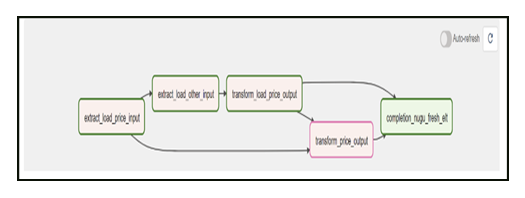
\includegraphics[width =4.5cm]{pictures/picture5.eps}
    \hfil
\caption{Overall Airflow Dag configuration diagram}
\end{figure}

\begin{table}[!htbp]
\begin{tabular}{|l|l|l|}
\hline
Directory & File names                                                                                              & Module names in use \\ \hline
/dags &
  \begin{tabular}[c]{@{}l@{}}nugu\_fresh\_dag.py,\\ nugu\_fresh.py\end{tabular} &
  \begin{tabular}[c]{@{}l@{}}airflow, keras, \\ requests,joblib\end{tabular} \\ \hline
/iscalers &
  \begin{tabular}[c]{@{}l@{}}input1\_scaler.pkl,\\  input2\_scaler.pkl,   \\ input3\_scaler.pkl, \\ input4\_scaler.pkl,\\ input5\_scaler.pkl\end{tabular} &
  - \\ \hline
/tscalers &
  \begin{tabular}[c]{@{}l@{}}target1\_scaler.pkl,\\ target2\_scaler.pkl,\\ target3\_scaler.pkl, \\ target4\_scaler.pkl,   \\ target5\_scaler.pkl\end{tabular} &
  - \\ \hline
/models   & \begin{tabular}[c]{@{}l@{}}model1.h5,\\ model2.h5,\\ model3.h5, \\ model4.h5, \\ model5.h5\end{tabular} & -                   \\ \hline
\end{tabular}
\end{table}
\paragraph{/dags}
dags folder contains functions that extract, predict, load fresh product data. ‘nugu\_fresh\_dag.py’ determines the order in which each task is executed according to its dependency. ‘nugu\_fresh.py’ contains specific instructions written in Python for each task. Each task is connected to the database and given an appropriate role. The ‘requests’ module is used to extract data using API, the ‘joblib’ module is used to load pre-written sklearn MinMaxscalers to preprocess data, and the ‘keras’ module is used to predict data by calling a pre-written deep learning model. Tasks are connected to the database using 'airflow' and determine the overall order of tasks.

\paragraph{/iscalers}
Iscaler folders contain pre-produced sklearn MinMaxscalers for input data of deep learning model in pkl file format. These files are used by Airflow to preprocess and restore data to its original format, and are loaded using the joblib module.

\paragraph{/tscalers}
tscaler folders contain pre-produced sklearn MinMaxscalers for ouput data of deep learning model in pkl file format. These files are used by Airflow to restore data to its original format, and are loaded using the joblib module.

\paragraph{/models}
models folders contain pre-produced Keras deep learning model in h5 file format. These files are used by Airflow to predict price of fresh product.

\subsubsection{Backend}

\begin{table}[!htbp]
\begin{tabular}{|l|l|l|}
\hline
Directory & File names                                                                                            & Module names in use \\ \hline
/nugu\_fresh &
  \begin{tabular}[c]{@{}l@{}}settings.py, urls.py,\\ wsgi.py\end{tabular} &
  \begin{tabular}[c]{@{}l@{}}Django,\\ Django Rest \\ Framework\end{tabular} \\ \hline
/api &
  \begin{tabular}[c]{@{}l@{}}models.py, urls.py, \\ views.py,   \\ crawlers.py\end{tabular} &
  \begin{tabular}[c]{@{}l@{}}Django, \\ Django \\ Rest Framework\end{tabular} \\ \hline
-         & \begin{tabular}[c]{@{}l@{}}gitignore, \\ db.sqlite3,   \\ manage.py, \\ requirements.txt\end{tabular} & Django              \\ \hline
\end{tabular}
\end{table}

\paragraph{/nugu_fresh}
When utilizing the Django framework, an app directory, that has the same name of a project directory, must be created. Inside the directory, there are settings.py, which manage settings for the django server and nugu settings.py, where private data such as secret keys are stored.

\paragraph{/api}
Django module and crawler functions are used in this directory. ‘models.py’ makes DB table, ‘urls.py’ handles routing for NUGU actions. ‘views.py’ gets request from NUGU and response which is contextual. ‘crawlers.py’ return the lowest value from three different early morning delivery company.   

\paragraph{SQLite}
SQLite is a database management system such as MySQL and PostgreSQL, but it is a relatively light database for use in response programs, not servers. Python provides the SQLite library as a standard bundled element with the basic version of the Python interpreter.

\section{USE CASES}
\begin{figure}[h]
\centering
    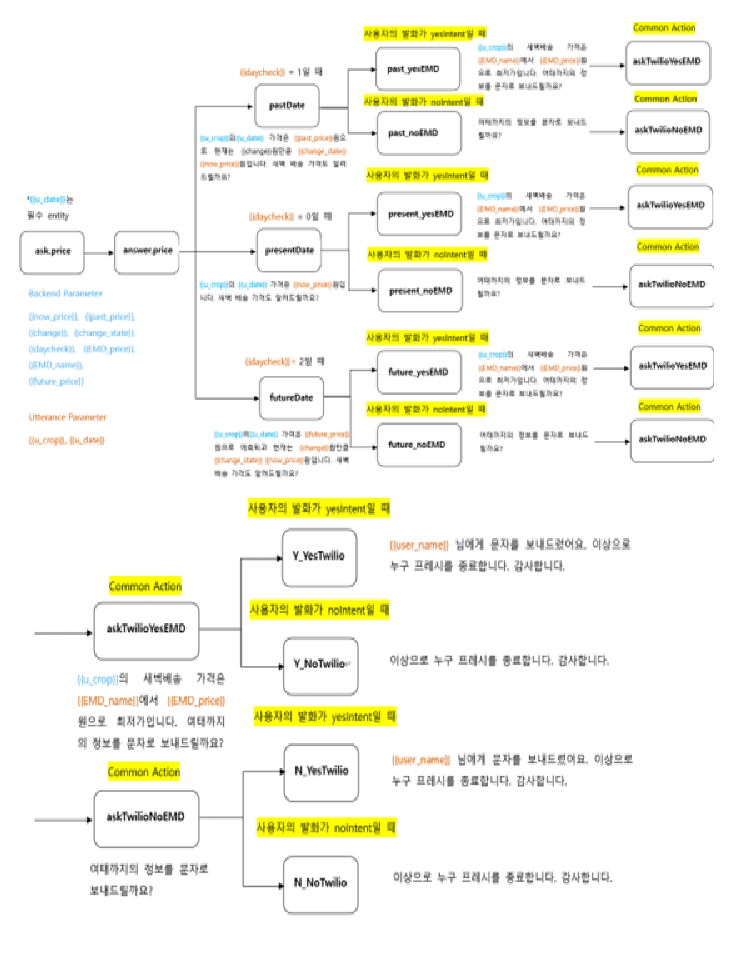
\includegraphics[width =4.5cm]{pictures/picture6.eps}
    \hfil
\caption{Overall Usecase}
\end{figure}

\subsection{Return historical price}
% Please add the following required packages to your document preamble:
% \usepackage{multirow}
\begin{table}[!htbp]
\begin{tabular}{|l|l|l|}
\hline
발화 주체 &
  대표 발화 &
  기능 \\ \hline
USER &
  “아리야, 프레시 시작” &
  \multirow{2}{*}{\begin{tabular}[c]{@{}l@{}}\#0. 누구프레시 \\ 실행\end{tabular}} \\ \cline{1-2}
NUGU &
  \begin{tabular}[c]{@{}l@{}}“안녕하세요. 누구 \\ 프레시입니다. 무엇을 \\ 도와드릴까요?”\end{tabular} &
   \\ \hline
USER &
  “어제 배추 가격 알려줘” &
  \multirow{2}{*}{\begin{tabular}[c]{@{}l@{}}\#1. \\    \\ 과거 가격 \\ 알림\end{tabular}} \\ \cline{1-2}
NUGU &
  \begin{tabular}[c]{@{}l@{}}“배추의 어제 가격은 \\ OOO원으로 현재는 \\ OO원 비싼 \\ OOO원입니다.”\end{tabular} &
   \\ \hline
NUGU &
  \begin{tabular}[c]{@{}l@{}}“새벽 배송 가격도 \\ 알려드릴까요? 원하시면 \\ ‘알려줘’, 원하지 \\ 않으시면 ‘아니’ 라고 \\ 말해주세요. 다시 \\ 들으시려면 ‘다시’ 라고 \\ 말해주세요.”\end{tabular} &
  \multirow{3}{*}{\begin{tabular}[c]{@{}l@{}}\#4. \\    \\ 새벽 배송 \\ 가격 알림\end{tabular}} \\ \cline{1-2}
USER &
  “알려줘” &
   \\ \cline{1-2}
NUGU &
  \begin{tabular}[c]{@{}l@{}}“배추의 새벽배송 가격은  \\ 쿠팡에서 XXXXX원으로   \\ 최저가입니다.”\end{tabular} &
   \\ \hline
NUGU &
  \begin{tabular}[c]{@{}l@{}}“여태까지의 정보를 \\ 문자로 보내드릴까요? \\ 원하시면 ‘보내줘’라고, \\ 원하지 않으시면 \\ ‘아니’라고 말해주세요. \\ 다시 들으시려면 \\ ‘다시’라고 말해주세요.”\end{tabular} &
  \multirow{3}{*}{\begin{tabular}[c]{@{}l@{}}\#5. \\    \\ 문자 발송 \\ 서비스\end{tabular}} \\ \cline{1-2}
USER &
  “보내줘” &
   \\ \cline{1-2}
NUGU &
  \begin{tabular}[c]{@{}l@{}}“사용자님에게 문자를 \\ 보내 드렸어요. 이상으로 \\ 프레시를   종료합니다. \\ 감사합니다.”\end{tabular} &
   \\ \hline
\end{tabular}
\end{table}
Allows users to receive a return of the historical price of the agricultural products. When a user requests to return the price at a specific point in the past, such as "Tell me the price of rice a week ago," after executing "Nugu Fresh," the speaker returns the price. This feature can only return prices up to the last week

\subsection{Return current price}
% Please add the following required packages to your document preamble:
% \usepackage{multirow}
\begin{table}[h]
\begin{tabular}{|l|l|l|}
\hline
발화 주체 &
  대표 발화 &
  기능 \\ \hline
USER &
  \begin{tabular}[c]{@{}l@{}}“아리야, 프레시 \\ 시작”\end{tabular} &
  \multirow{2}{*}{\begin{tabular}[c]{@{}l@{}}\#0. 누구프레시 \\ 실행\end{tabular}} \\ \cline{1-2}
NUGU &
  \begin{tabular}[c]{@{}l@{}}“안녕하세요. 누구 \\ 프레시입니다. \\ 무엇을 \\ 도와드릴까요?”\end{tabular} &
   \\ \hline
USER &
  \begin{tabular}[c]{@{}l@{}}“오늘 배추 가격 \\ 알려줘”\end{tabular} &
  \multirow{2}{*}{\begin{tabular}[c]{@{}l@{}}\#2.\\    \\ 현재 가격\\    \\ 알림\end{tabular}} \\ \cline{1-2}
NUGU &
  \begin{tabular}[c]{@{}l@{}}“오늘 서울 배추의 \\ 가격은 OOO원 \\ 입니다.”\end{tabular} &
   \\ \hline
NUGU &
  \begin{tabular}[c]{@{}l@{}}“새벽 배송 가격도 \\ 알려드릴까요? \\ 원하시면 ‘알려줘’, \\ 원하지 않으시면 \\ ‘아니’ 라고 \\ 말해주세요. 다시 \\ 들으시려면 ‘다시’ \\ 라고 말해주세요.”\end{tabular} &
  \multirow{3}{*}{\begin{tabular}[c]{@{}l@{}}\#4.\\    \\ 새벽 배송 가격 \\ 알림\end{tabular}} \\ \cline{1-2}
USER &
  “알려줘” &
   \\ \cline{1-2}
NUGU &
  \begin{tabular}[c]{@{}l@{}}배추의 새벽배송 \\ 가격은 쿠팡에서 \\ XXXXX원으로 \\ 최저가입니다.\end{tabular} &
   \\ \hline
NUGU &
  \begin{tabular}[c]{@{}l@{}}“여태까지의 정보를 \\ 문자로 \\ 보내드릴까요? \\ 원하시면 \\ ‘보내줘’라고, \\ 원하지 않으시면 \\ ‘아니’라고 \\ 말해주세요. \\ 다시 들으시려면\\ ‘다시’라고 \\ 말해주세요.”\end{tabular} &
  \multirow{3}{*}{\begin{tabular}[c]{@{}l@{}}\#5. \\    \\ 문자 발송\\    \\ 서비스\end{tabular}} \\ \cline{1-2}
USER &
  “보내줘” &
   \\ \cline{1-2}
NUGU &
  \begin{tabular}[c]{@{}l@{}}“사용자님에게 \\ 문자를 보내 \\ 드렸어요. \\ 이상으로 프레시를   \\ 종료합니다. \\ 감사합니다.”\end{tabular} &
   \\ \hline
\end{tabular}
\end{table}
Allows users to return the current price of agricultural products. If you request the price of a particular agricultural product the speaker receives the price of the agricultural product in real time and returns it to the user.

\subsection {Return future price}
% Please add the following required packages to your document preamble:
% \usepackage{multirow}
{
\begin{table}[h]
\begin{tabular}{|l|l|l|}
\hline
발화 주체 &
  대표 발화 &
  기능 \\ \hline
USER &
  “아리야, 프레시 시작” &
  \multirow{2}{*}{\begin{tabular}[c]{@{}l@{}}\#0. 누구프레시 \\ 실행\end{tabular}} \\ \cline{1-2}
NUGU &
  \begin{tabular}[c]{@{}l@{}}“안녕하세요. 누구 \\ 프레시입니다. 무엇을 \\ 도와드릴까요?”\end{tabular} &
   \\ \hline
USER &
  \begin{tabular}[c]{@{}l@{}}“내일 배추 가격 \\ 알려줘”\end{tabular} &
  \multirow{2}{*}{\begin{tabular}[c]{@{}l@{}}\#3. 미래 가격 \\    \\ 알림\end{tabular}} \\ \cline{1-2}
NUGU &
  \begin{tabular}[c]{@{}l@{}}“배추의 내일 \\ 가격은OOO원으로 \\ 예측되고 현재는 \\ OO원 비싼 OOO 원 \\ 입니다.”\end{tabular} &
   \\ \hline
NUGU &
  \begin{tabular}[c]{@{}l@{}}“새벽 배송 가격도 \\ 알려드릴까요? \\ 원하시면 ‘알려줘’, \\ 원하지 않으시면 \\ ‘아니’ 라고 \\ 말해주세요. \\ 다시 들으시려면 \\ ‘다시’ 라고 \\ 말해주세요.”\end{tabular} &
  \multirow{3}{*}{\begin{tabular}[c]{@{}l@{}}\#4. 새벽 배송 \\ 가격 알림\end{tabular}} \\ \cline{1-2}
USER &
  “알려줘” &
   \\ \cline{1-2}
NUGU &
  \begin{tabular}[c]{@{}l@{}}“배추의 새벽배송 \\ 가격은  쿠팡에서 \\ XXXXX원으로   \\ 최저가입니다.”\end{tabular} &
   \\ \hline
NUGU &
  \begin{tabular}[c]{@{}l@{}}asks “여태까지의 \\ 정보를 문자로 \\ 보내드릴까요? \\ 원하시면 \\ ‘보내줘’라고, 원하지 \\ 않으시면 ‘아니’라고 \\ 말해주세요. 다시 \\ 들으시려면 ‘다시’라고   \\ 말해주세요.”\end{tabular} &
  \multirow{3}{*}{\begin{tabular}[c]{@{}l@{}}\#5. \\    \\ 문자 발송 \\ 서비스\end{tabular}} \\ \cline{1-2}
USER &
  “보내줘” &
   \\ \cline{1-2}
NUGU &
  \begin{tabular}[c]{@{}l@{}}사용자님에게 문자를 \\ 보내 드렸어요. \\ 이상으로 프레시를 \\ 종료합니다. \\ 감사합니다\end{tabular} &
   \\ \hline
\end{tabular}
\end{table}
}
User can respond to the future prices of agricultural products. When a user asks NUGU FRESH to give a specific point-in-time price of a particular agricultural product, NUGU FRESH returns a future predictor of that agricultural product based on the learning results. The return value may differ from the real price. These features are compatible with Requirement A-2.

\subsection{Notification the price of early-morning delivery service}
Users can receive a current price notification for early morning delivery services after a price notification. If the user wants to know the price of the early morning delivery service, "NUGU FRESH" crawls the price of companies that support early morning delivery in real time and returns the price of the company and its agricultural products which offers lowest price.

\subsection{Text service}
If a user links its mobile phone with NUGU Fresh, the user can receive the results back to its mobile phone. After each of the functions NUGU Fresh asks the user to send the response value by text, and if the user wants to receive it, the results are sent to the linked phone.

\section{Discussion}
\subsection{Difficulties}
    Agricultural price prediction is one of the time series predictions, predicting the future through historical data observed sequentially over time. These time series predictions had difficulty in selecting prediction models based on the agricultural product price data held because the appropriate time series prediction models were different depending on the characteristics of the data and there were no clear criteria for which model was more suitable for each characteristic. In particular, in the case of agricultural price data we deal with, there were so many variables that could affect prices like temperature, wind speed, prices, oil prices, output from the previous year, prices from the previous year, etc. In addition, it was not easy to make accurate predictions because the degree to which these various variables affect future price predictions was different and the degree of correlation between some of these variables was high. To solve this problem, variables that affect crop prices were selected based on several papers, and these variables were collected to obtain correlation values between variables, excluding variables that exceed certain values.
    Outside of technology, we had difficulty in deciding the first topic and distributing roles to our team members. Basically, because we had to use AI, we had to choose a topic that could use AI well, but all four of the team members were not familiar with AI, so it was difficult to select a topic suitable for using AI. In addition, because what kind of people we were going to be targeting and whether the people really needed it were a very important factor for the service we were going to create, we consulted the people around us and read the related papers to select the topic.
    In terms of role allocation, as we said earlier, it was everyone's first time experiencing AI, so we were very worried about who would be in charge of the AI part. At first, we just tried to do AI parts together and distribute the rest of the parts, but when we tried to do that, we thought it was too inefficient for the four of us to study and repeat the same AI part, and we thought that we would not be able to finish it in a short time. Eventually, we assigned team members who handled well in the rest of the parts except for AI parts first and left AI parts to the remaining team members so that the project could be done more efficiently.
\subsection{Scalabilities}
\begin{figure}[h]
\centering
    
\includegraphics[width =8cm]{pictures/picture7.eps}
    \hfil
\caption{NUGU App’s functions}
\end{figure}
    In this project, we provided NUGU FRESH service for only five crops: potatoes, onions, radishes, cabbages, and rice, but it was a bit disappointing because there seemed to be few crops handled during the project. Therefore, we thought that it could be widely used for more people if the service was not only limited to five crops, but also included various crops and high-consumption fruits. In addition, NUGU APP's functions such as menu recommendation and recipe were linked to select agricultural products that could be reasonably consumed through the services provided by NUGU FRESH, and if they could receive menu recommendations and recipes, they would provide more advanced services to NUGU speaker users. Moreover, with the current service, we could only send the information requested by the user by text, but we thought it would be better to print this information out.\\
    \\
    
    \centering
    REFERENCES
[1]https://developers-doc.nugu.co.kr/nugu-play/create-plays-with-play-builder
[2]https://tykimos.github.io/lecture/

\end{document}%%
